\section{Dettagli}
In questa sezione si affrontano in maniera più dettagliata le principali funzionalità
offerte dal microservizio. In letteratura (es: \cite{7030212}, \cite{8229914}) vi è un ampio
dibattito su quale sia
l'effettiva dimensione di un microservizio, e di fatto si dice che esso
dovrebbe fare una cosa ed una soltanto. Si potrebbe quindi dire che questo principio
non è completamente rispettato in \texttt{MoonCloud\_VPN}. A tale proposito, vanno fatte
le seguenti osservazioni:
\begin{itemize}
	\item il microservizio nella sua interezza non è particolarmente complesso, anche
	      dal punto di vista algoritmico, a parte il trasferimento file ed il mappaggio
	      delle reti il codice è abbastanza semplice. 
	      Si tratta di circa 4000 righe di codice Python, escludendo i test ed ulteriori script,
	      che è una dimensione ragionevole.
	\item Il microservizio svolge una precisa funzionalità, ovvero gestire tutto ciò
	      che riguarda la configurazione di OpenVPN  per MoonCloud.
\end{itemize}
Queste considerazioni hanno portato a lasciare questo microservizio come un \textit{unico}
microservizio.

\subsection{Certificate Management}
Requisito fondamentale per il funzionamento di OpenVPN è che client e server dispongano
di certificati X509 firmati da una stessa CA.
A tale scopo, si dispone di una CA interna, la cui chiave pubblica e privata è deployata
assieme a questo servizio\footnote{In futuro si adotteranno misure di protezione per la
	chiave privata, oltre alla protezione \textit{fisica} (es: regole di firewall) dell'accesso
al servizio.}. Attualmente il certificato è self-signed, in futuro potrebbe non essere così.

OpenVPN richiede, sia per client sia per server, che siano settati alcuni attributi
specifici nei certificati, da cui poi derivano le direttive
``\texttt{remote-cert-eku "TLS Web Server/Client
Authentication"}''. Ogni certificato ha un seriale univoco, il quale viene generato
in maniera pseudocasuale usando una funzione preposta dalla libreria che viene
utilizzata.

Il microservizio mantiene anche una CRL -- \textit{Certificate Revocation List}, la quale
contiene l'elenco dei seriali dei certificati revocati, la ragione (nel cui caso è ``\texttt{unspecified}''),
ed è firmata digitalmente dalla chiave privata della CA.\\
Ogni volta che si revoca un nuovo client, occorre creare una nuova CRL inserendo tutti i
precedenti certificati revocati ed aggiungendo quello del client in questione. La CRL deve
poi essere distribuita 
a tutti i server, ma questo è compito di un altro modulo.

I certificati sono generati utilizzando l'algoritmo \texttt{ECDSA}, con livello di sicurezza
128 bit per client e server. Secondo le raccomandazioni del NIST, un livello di sicurezza di
128 bit è sicuro fino al 2030 \cite{Barker:2016:SRK:2206273}. Si può passare senza
problemi ad un livello di sicurezza maggiore (192 o 256), semplicemente modificando i settaggi
del microservizio.

Per il certificato della CA, si utilizza invece una curva ellittica con livello di sicurezza
di 256 bit.


Tutto il codice per la gestione di queste funzionalità è implementato nel modulo \texttt{openssl}
mediante il file \texttt{openssl.py}, di cui di seguito si mostra un estratto leggermente
modificato.
Si può vedere come si crea un certificato ed una CRL vuota (metodo
``\texttt{create\_empty\_crl}'', per la quale vi
si aggiunge un certificato \textit{fake} il cui numero seriale vale 1 (questo per avere una
CRL che contenga almeno un certificato, ed evitare problemi con CRL vuote).
Il tipo di certificato (client o server), dipende dai parametri con cui si chiama il metodo
``\texttt{create\_keys\_and\_cert}''.
Alcuni metodi sono omessi per brevità, tra essi il costruttore.
\inputminted[tabsize=4, breaklines, fontsize=\footnotesize]{python}{code_samples/openssl.py}


Nel database si memorizzano anche informazioni relative ai certificati, come il
\texttt{CommonName}, il seriale, il livello di sicurezza, l'algoritmo
di firma. Questa tabella è quindi referenziata dalla relativa
tabella che rappresenta i VPN server ed i VPN device client.

Si mantiene anche un tabella con informazioni relative alla CRL, come la data di ultima
modifica.


\subsection{IP Mapping}
L'IP Mapping è una funzionalità fondamentale per poter far sì che un VPN server possa
gestire il maggior numero possibile di reti target diverse.
Durante l'analisi dei requisiti è stato osservato che
gli Execution Manager dedicati all'analisi di reti target sono posti
ciascuno in una rete isolata rispetto al resto di MoonCloud, ciò ha portato
alle seguenti conclusioni:
\begin{itemize}
	\item è possibile assegnare più volte la stessa rete mappata a diversi client,
	      a patto che siano collegati a VPN server diversi, e quindi Execution Manager.
	\item E' possibile assegnare \textit{qualsiasi} indirizzo IP, non solo quell
	      indicati come \textit{privati}, questo perché tali indirizzi sono utilizzati
	      sono nel contesto degli Execution Manager. Per evitare eventuali conflitti,
	      come ad esempio assegnare una rete mappata che contiene l'indirizzo IP
	      di una repository Linux, deve essere possibile poter escludere degli indirizzi,
	      reti, nomi di dominio.
\end{itemize}

\subsubsection{Assegnamento reti}
Il grafico \ref{fig:sequence-mapping-assign} rappresenta, mediante la notazione UML per
i diagrammi di interazione, quali azioni sono svolte per l'assegnamento delle reti, che
qui viene descritto a parole.
\begin{enumerate}
	\item Per ciascuna rete in input da mappare, si crea un corrispondente oggetto (detto
	      ``\textit{rete canonica}'') che
	      ha come subnet mask una subnet mask \textit{classful} in grado di contenere tutti
	      gli indirizzi della rete in input. Ad esempio, se in input vi è una rete con subnet
	      mask a 26 bit, il corrispettivo oggetto è una rete con lo stesso NET ID e con
	      subnet mask a 24 bit.
	\item Si raggruppano tutte le reti canoniche per subnet mask.
	\item Per ciascun gruppo, si richiede al databse un numero di reti mappate pari
	      al numero di reti che costituiscono ciascun gruppo.
	\item Si utilizza una funzione
	      (il DBMS PostgreSQL consente di farlo) salvata nel database per questa operazione,
	      poiché si devono effettuare numerose query. Facendo tutto con una funzione nel database,
	      si richiede meno I/O. La funzione garantisce che le reti mappate che vengono
	      infine ritornate non siano nella blacklist. Si noti che grazie ai tipi di dati
	      \texttt{INET}  e \texttt{CIDR}, certe interrogazioni sono molto efficienti
	      (ad esempio esiste un operatore per valutare se un indirizzo IP è contenuto in una
	      rete).
	\item Si \textit{allineano} le reti in input con le reti mappate, e le si salvano
	      nel database.
	\item Si effettua un secondo allineamento tra le reti mappate e quelli in input,
	      ritornando infine una lista di oggetti che contengono tutte le informazioni
	      per creare il file di script per nftables.
\end{enumerate}
Si noti che nel database si salvano, di fatto, delle coppie \texttt{Rete Originale -- Rete Mappata}.
Si può vedere un indirizzo IP originale come l'offset tra esso e il NET ID, ed
allo steso modo, il corrispondente indirizzo mappato si calcola sommando l'offset dell'IP
originale al NET ID mappato.

La creazione del mapping è abbastanza complessa, si inserisce come codice d'esempio
la creazione del file di script per nftables.
\inputminted[tabsize=4, breaklines, fontsize=\footnotesize]{python}{code_samples/nftables.py}

\begin{figure}
	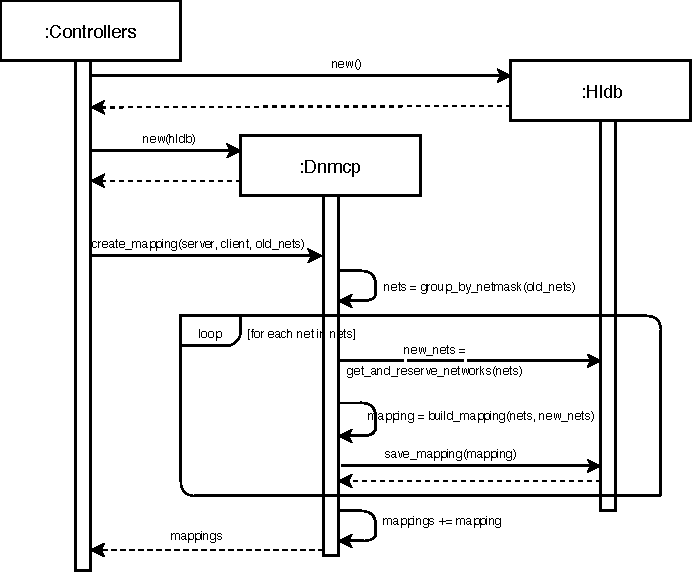
\includegraphics[scale=0.65]{img/sequence_mapping}
	\caption[Diagramma di interazione: assegnamento reti]{Diagramma di interazione che mostra
		le chiamate tra le vari classi che collaborano per assegnare nuove reti mappate
		all'aggiunta di un nuovo client (altre azioni, come la creazione dei file di configurazione
		vengono omesse). La classe \texttt{HLDB} si occupa dell'interazione con il database, mentre
		\texttt{DNMCP} compie operazioni ad un più alto livello.}
	\label{fig:sequence-mapping-assign}
\end{figure}

\subsubsection{Ritornare indirizzo IP mappato}
Quando un client specifica un target per un'analisi, egli lo fà inserendo l'indirizzo
IP originale, per lui la questione dell'IP mapping è completamente trasparente. Ciò
significa che occorre una funzione che, dato un indirizzo IP originale di un
certo VPN client, ritorni quello mappato, poiché esso è l'unico noto a MoonCloud.
Tale funzione viene implementata dal microservizio, ed è molto performante.
I passi da compiere sono:
\begin{itemize}
	\item fare una query al database e ritornare la rete mappata cui corrisponde
	      la rete originale a cui appartiene l'indirizzo IP richiesto in input.
	      Anche in questo caso si sfruttano gli operatori specifici messi a disposizione
	      dal DBMS.
	\item Il corrispondente IP mappato si calcola con i seguenti step:
	      \begin{itemize}
	      	\item applicare la subnet mask al NET ID originale ed all'IP originale,
	      	      la subnet mask è memorizzata nel database.
	      	\item Applicare la subnet mask al NET ID mappato o al primo indirizzo IP
	      	      della rete mappata in caso non sia il NET ID (ad esempio: il mapping
	      	      parte da \texttt{192.168.100.10} anziché \texttt{192.168.100.0}).
	      	\item Calcolare l'offset dell'indirizzo IP originale sottraendo
	      	      l'IP originale con la subnet mask applicata al NET ID originale
	      	      con la subnet mask applicata.
	      	\item Sommare l'offset all'indirizzo IP mappato di partenza con
	      	      la subnet mask applicata.
	      \end{itemize}
\end{itemize}
Le operazioni potrebbero essere effettuate anche senza l'applicazione della
subnet mask, si tenga comunque conto che applicare una subnet mask
ad indirizzo IP equivale ad un AND logico, quindi un'istruzione in ogni
caso molto veloce.


\subsection{Trasferimento file}
Vi sono diverse situazioni che richiedono il trasferimento di file
verso i VPN server di MoonCloud. Qualsiasi sia il caso, esso viene effettuato
usando il protocollo SSH, mediante il quale si possono sia inviare comandi remoti
o trasferire file con il sottosistema SFTP -- Secure File Transfer Protocol. Si sfruttano
delle librerie Python a tale scopo. L'autenticazione viene fatta mediante chiave
pubblica.
Il trasferimento è richiesto nelle seguenti situazioni:
\begin{description}
	\item[Creazione di un nuovo server]Si trasferiscono sul server il file
	di configurazione principale di OpenVPN, la relativa chiave privata e certificato,
	la chiave pubblica della CA, la CRL.
	Vengono trasferiti anche due script:
	\begin{itemize}
		\item \texttt{move\_files\_server.py}: dopo aver trasferito i file appena elencati
		      in una cartella sul server, viene lanciato questo script, il quale legge il file
		      di configurazione principale e da esso deduce la struttura di directory e file
		      richiesta, e quindi la crea.
		      Poiché le operazioni che lo script deve compiere non sono poche, si è
		      preferito scegliere questa strada anziché invocare direttamente $n$ commandi 
		      lungo la connessione SSH per ridurre l'I/O e quindi aumentare le prestazioni.
		\item \texttt{deleteclient.py}. Quando si revoca un client, esso deve essere
		      \textit{totalmente eliminato}, ciò si traduce anche nell'eliminare ogni riferimento
		      ad esso dai file \texttt{client-up.sh} e \texttt{client-down.sh}, quindi eliminare
		      il corpo degli \texttt{if} all'interno dei due file. Questa operazione viene
		      svolta direttamente sui server, mediante l'invocazione di questo script.
		      Analogamente a quanto detto per lo script precedente, e a maggior ragione in questo
		      caso, eseguire \texttt{deleclient.py} direttamente sul server riduce di molto l'I/O:
		      se non si fosse scelta questa opzione sarebbe stato necessario trasferire i due file,
		      modificarli, e di nuovo caricarli sul server.
	\end{itemize}
	\item[Creazione di un nuovo client]E' necessario creare un file con lo stesso
	nome del \texttt{CommonName} presente nel certificato del client, il cui
	contenuto è la direttiva ``\texttt{iroute}''\footnote{Si rimanda al capitolo dedicato
	alle configurazioni di OpenVPN.}. Esso deve essere quindi trasferito in una cartella
	specifica nel VPN server. Oltre a tale file, è necessario modificare gli script
	\texttt{client-up.sh} e \texttt{client-down.sh}, aggiungendo un nuovo ramo
	\texttt{if} specifico per questo client.
	\item[Rinnovo certificato server]L'unico trasferimento da effettuare è il nuovo
	certificato e chiave pubblica, i quali devono essere spostati nella directory
	specificata, ancora una volta, nel file di configurazione di OpenVPN nel server.
	Rimane comunque la necessità di riavviare il server affinché questi cambiamenti abbiano
	effetto.
	\item[Rinnovo certificato client]E' necessario revocare il certificato precedente,
	quindi propagare la nuova CRL ad ogni server di MoonCloud.
	\item[Revoca certificato client]Occorre aggiornare e distribuire la
	CRL ed invocare \\\texttt{deleteclient.py} sul server a cui quel client si collegava (oltre
	ad eliminare i dati inerenti al client dal database).
	\item[Refresh CRL]Quando si crea una CRL si specifica la data di prossimo aggiornamento,
	ed essa viene controllata da OpenVPN server: se risulta scaduta non si accettano nuove
	connessioni. Per questa ragione è importante aggiornarla, ovvero creare una nuova
	CRL che contenga gli stessi certificati revocati della precedente ma con
	data di prossimo aggiornamento posticipata di un anno.
\end{description}

Il trasferimento dei file verso i server è una parte fondamentale del microservizio,
pertanto deve essere il più possibile robusto.
Il modo in cui viene effettuato è stato chiamato \textbf{\textit{asynchronous transferring}},
perché è svolto da due thread specifici a questo scopo, separati dagli altri thread di
esecuzione, implementati dalla classe \texttt{SSHBackgroundWorker}.
Il modulo \texttt{controllers} organizza i trasferimenti da effettuare e crea degli
oggetti (\textit{dizionari} Python) e li deposita su una delle due code condivise con i
thread di trasferimento.
La computazione di \texttt{SSHBackgroundWorker} è composta da due loop (uno per ogni thread), dentro
il quale si estraggono elementi dalla coda: ciascun elemento estratto contiene tutte le informazioni
che servono per trasferirlo sul server (o sui server) correttamente. I trasferimenti
quindi sono eseguiti serialmente, nell'ordine con cui sono stati inseriti
in una delle due code (\textit{FIFO}).
Ogni volta che si deposita un nuovo job sulla coda, si riceve un \texttt{WorkID}, il quale
è generato in maniera pseudocasuale allo scopo di identificare univocamente ogni job.

Lo stato della computazione di un lavoro è mantenuto in memoria da Redis. Tra le varie informazioni
che si memorizzano vi sono:
\begin{itemize}
	\item ID del lavoro (è la Key)
	\item stato di avanzamento: non iniziato (``\texttt{Pending}''), in corso (``\texttt{Working}''),
	      concluso (``\texttt{Executed}''), concluso con errore (``\texttt{Error}'')
	\item tipo (es: \textit{trasferimento server}, \textit{rinnovo certificato}, ecc\ldots)
	\item ulteriori informazioni, come una descrizione dell'errore in caso si verifichi.
\end{itemize}

Quando un thread inizia la computazione per un job modifica lo stato da \texttt{Pending}
a \texttt{Working}, infine ad \texttt{Executed} quando è finito.

Inizialmente si utilizzava, al posto di Redis, un dizionario acceduto concorrentemente dai thread,
tuttavia questo richiedeva un elevato uso di meccanismi di lock. Si è deciso quindi di
passare a Redis, il quale, in quanto database di tipo Key--Value, è molto efficiente,
inoltre tutte le operazioni svolte da esso sono atomiche per definizione.
Inoltre, per le interrogazioni più complesse, è possibile definire degli script Lua
e richiamarne quindi la loro esecuzione; più avanti se ne mostra un esempio.

Una volta che il job è stato depositato in una coda dal \texttt{controllers}, si ritorna immediatamente
la risposta HTTP, tale risposta contiene anche lo \texttt{WorkID}. E' responsabilità
del chiamante fare quindi del \textit{polling} al microservizio per verificare se il task
si è concluso. Tali richieste si traducono in una interrogazione a Redis.

Quando si richiede lo stato di un lavoro ed esso è stato completato, viene rimosso da Redis.

La ragione per cui il trasferimento segue questo paradigma non è prestazionale, bensì è per
garantire l'integrità dei file sui server.
Si pensi ad un semplice esempio, per cui si fanno due richieste a questo microservizio nello stesso
momento, ed entrambe richiedono di aggiungere un nuovo client allo stesso server.
Si supponga che vi siano due thread, ciascuno che gestisce una delle due risposte. Essi quindi
accedono al file \texttt{client-down.sh} (e \texttt{client-up.sh}) sul server, lo modificano
aggiungendo informazioni
relative solo al proprio client, quindi il primo thread trasferisce il file, immediatamente dopo
il secondo trasferisce la propria versione, ed ecco che la modifica fatta dal primo viene
sovrascritta.

Un altro problema a cui si può pensare è il seguente: si fà una richiesta di revoca di un certificato,
la CRL viene quindi modificata ed inizia la propagazione verso tutti i server.
Poi si fà una richiesta di refresh, quindi la si ricrea ed inizia la distribuzione\ldots Qua c'è il
problema. Se si suppone che in totale vi siano 100 server e che la seconda richiesta sia arrivata
mentre si concludeva il trasferimento verso il 50esimo, a quel punto si modifica la CRL
e quella trasferita al 51esimo è diversa dalle precedenti.

Un'esecuzione seriale mette al sicuro da questi problemi.
Per ciò che concerne le modifiche alla CRL, esse stesse sono
schedulata in maniera seriale, non solo il suo trasferimento.


Inizialmente tutte le operazioni venivano eseguite da un unico thread, successivamente se ne
è aggiunto un secondo.
\begin{itemize}
	\item \texttt{Main\_worker\_thread} si occupa del trasferimento di nuovi server, nuovi
	      client e, parzialmente, della revoca di un client chiamando lo script di cancellazione
	      \texttt{deleteclient.py}.
	      Si noti che questo thread è l'\textit{unico} flusso di computazione che può modificare
	      i file \texttt{client-up.sh} e \texttt{client-down.sh}.
	\item \texttt{CRL\_worker\_thread} è responsabile dell'aggiornamento e della propagazione
	      della CRL ai diversi server. Anche in questo caso, vi è un unico flusso che modifica
	      un file, per cui l'integrità della CRL è ancora garantita.
\end{itemize}
L'unica operazione definibile problematica poiché coinvolge entrambi i due thread è la revoca
di un client, poiché occorre sia modificare i file \texttt{client-up.sh} e \texttt{client-down.sh}
sia aggiornare la CRL. In questo caso la soluzione adottata consiste nel dividere il lavoro in
entrambi i thread, il primo si occupa solo di chiamare \texttt{deleclient.py}, il secondo
di aggiornare e distribuire la CRL. Le strutture dati memorizzate da Redis sono organizzate in modo
da poter tener conto del progresso parziali di ciascun thread.


Di seguito si mostra un estratto di \texttt{SSHBackgroundWorker}, in particolare si mostrano
i due loop eseguiti dai due thread.

\inputminted[tabsize=4, breaklines, fontsize=\footnotesize]{python}{code_samples/sshworker_loops.py}

Il prossimo codice presentato è uno script Lua che viene eseguito su Redis\footnote{\url{https://www.lua.org/}}.
E' utilizzato
per ritornare, in una sola query a tale database, l'intera lista dei job.
Senza tale script, sarebbe stato necessario fare una prima query per ottenere la lista degli
\texttt{WorkID}, poi, per ciascuno di essi, richiedere l'oggetto completo.

\inputminted[tabsize=4, breaklines, fontsize=\footnotesize]{lua}{code_samples/works.lua}

\begin{figure}
	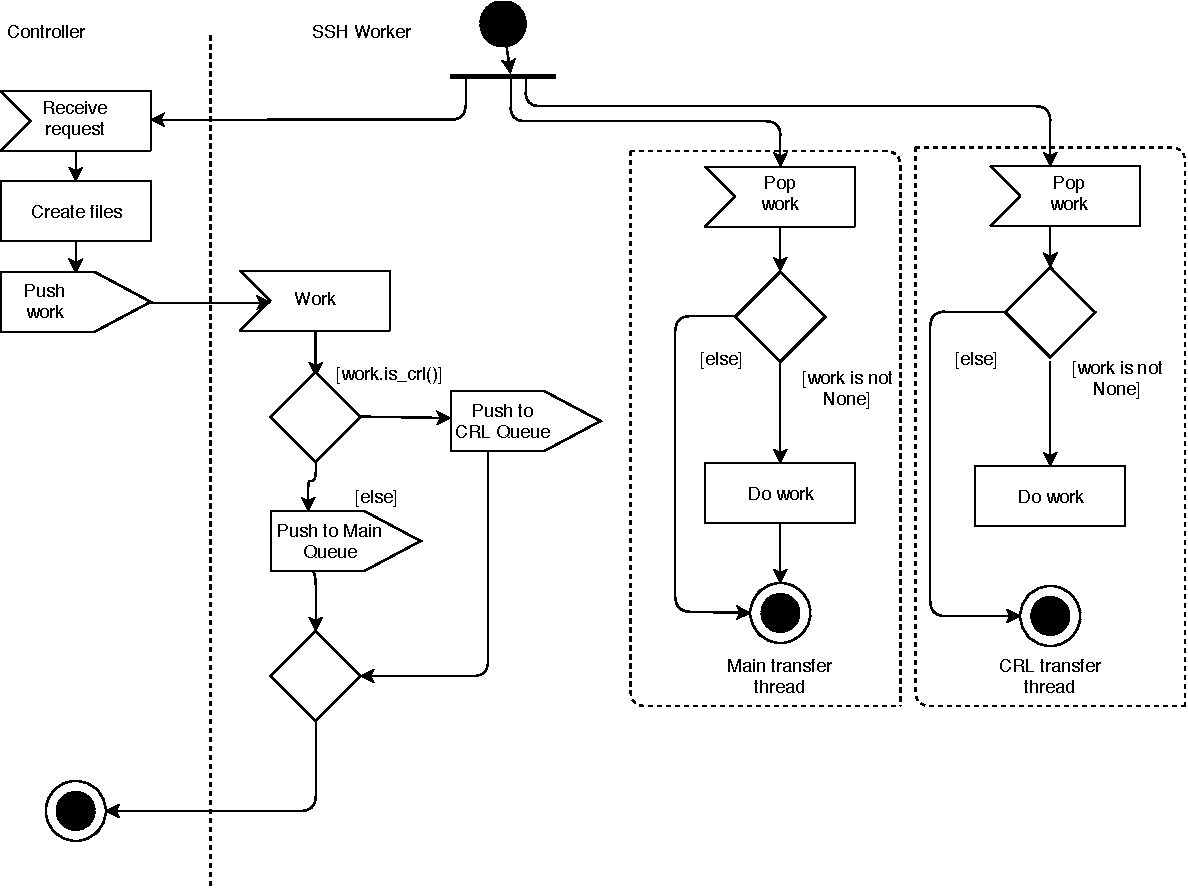
\includegraphics[scale=0.5]{img/activity_generic_file_transfer}
	\label{fig:activity-generic-file-transfer}
	\caption[Diagramma di attività: trasferimento file]{Diagramma di attività:
		trasferimento file. Il presente diagramma UML mostra cosa succede quando è necessario
		trasferire dei file. Ad una generica richiesta arrivata a \texttt{controllers},
		esso richiede di aggiungere un lavoro. Si decide quindi su quale coda
		depositarlo in base al tipo, quindi si ritorna al chiamante.
	Parallelamente, i due thread di trasferimento svolgono il lavoro.}
\end{figure}


\subsection{Registrazione server}
Registare un nuovo server significa che è stata già deployata in MoonCloud una VM dedicata
esclusivamente ad essere un VPN server, ed esso è raggiungibile anche dal Docker container su
cui si trova il microservizio \texttt{MoonCloud\_VPN}.
Viene messa a disposizione una API per questo scopo; i passi per creare un server sono:
\begin{enumerate}
	\item verificare che la chiave SSH fornita sia valida
	\item creare una nuova istanza nel database per il nuovo server
	\item creare i certificati ed i file di configurazione
	\item registrare nel database le informazioni relative al nuovo certificato
	\item mettere sulla coda di trasferimento un nuovo job, ovvero quello di
	      trasferire sul nuovo server tutti i file necessari.
\end{enumerate}
L'estratto di codice che si presenta ora è una versione leggermente modificata di ciò che
\texttt{controllers} fa.
\inputminted[tabsize=4, breaklines, fontsize=\footnotesize]{python}{code_samples/controllers_create_server.py}

Alla fine, la API ritorna al chiamante l'ID del server che lo identifica univocamente
nel database ed il \texttt{WorkID} relativo al trasferimento dei file. E' responsabilità
del chiamante fare ulteriori richieste per verificare lo stato del trasferimento. Per farlo
viene messa a disposizione una API specifica.

\subsection{Registrazione client}
Una API REST è predisposta alla creazione di un nuovo VPN device client. Tra gli input
che occorre fornire, è particolarmente importante specificare l'ID del server a cui
il client si connetterà e l'elenco delle reti che il client sarà in grado di
raggiungere una volta portato nella rete target.
Si compiono i seguenti step:
\begin{enumerate}
	\item fare un refresh della lista di nomi di dominio da escludere dal mapping
	\item creare una nuova istanza nel database per il device client
	\item creare i certificati ed i file di configurazione
	\item definire il mapping
	\item creare il file di script per nftables
	\item mettere sulla coda di trasferimento un nuovo job di tipo ``\texttt{Trasferire Client}''.
\end{enumerate}

Si ritorna al chiamante l'ID del client, il \texttt{WorkID} ed un file zippato codificato in formato
base64 che contiene:
\begin{itemize}
	\item file di configurazione principale per OpenVPN
	\item certificato e chiave privata del VPN client
	\item chiave pubblica della CA
\end{itemize}
Anche in questo caso si mostra un esempio.
\inputminted[tabsize=4, breaklines, fontsize=\footnotesize]{python}{code_samples/controllers_create_client.py}